\documentclass{article}
% Use the following version of the ``usepackage'' statement for
% submitting the draft version of the paper for review.  This will set
% the note in the first column to ``Under review.  Do not distribute.''
\usepackage{icml2007} 
\usepackage{times} 
% Use this version of the ``usepackage'' statement after the paper has
% been accepted, when creating the final version.  This will set the
% note in the first column to ``Appearing in''
%\usepackage[accepted]{icml2007}
\usepackage{code}
\usepackage{epsfig}
\usepackage{mlapa}
\newcommand{\cut}[1]{}

\newcommand{\appref}[1]{Appendix~\ref{#1}}
\newcommand{\secref}[1]{Section~\ref{#1}}
\newcommand{\tblref}[1]{Table~\ref{#1}}
\newcommand{\figref}[1]{Figure~\ref{#1}}
\newcommand{\listingref}[1]{Listing~\ref{#1}}
%\newcommand{\pref}[1]{{page~\pageref{#1}}}

\newcommand{\eg}{{\em e.g.}}
\newcommand{\cf}{{\em cf.}}
\newcommand{\ie}{{\em i.e.}}
\newcommand{\etc}{{\em etc.\/}}
\newcommand{\naive}{na\"{\i}ve}
\newcommand{\role}{r\^{o}le}
\newcommand{\forte}{{fort\'{e}\/}}
\newcommand{\appr}{\~{}}

\newcommand{\bftt}[1]{{\ttfamily\bfseries{}#1}}
\newcommand{\kw}[1]{\bftt {#1}}
\newcommand{\Pthen}{\kw{Pthen}}
\newcommand{\pads}{\textsc{pads}}
\newcommand{\padsl}{\textsc{padsl}}
\newcommand{\padst}{\textsc{pads/t}}
\newcommand{\datatype}{\textsc{PADS/T}}
%\newcommand{\datatype}{\textsc{DataType}}
\newcommand{\C}{\textsc{C}}
\newcommand{\perl}{\textsc{Perl}}
\newcommand{\ml}{\textsc{ml}}
\newcommand{\sml}{\textsc{sml}}
\newcommand{\smlnj}{\textsc{sml/nj}}
\newcommand{\java}{\textsc{java}}
\newcommand{\ddl}{\textsc{ddl}}
\newcommand{\xml}{\textsc{xml}}
\newcommand{\datascript}{\textsc{DataScript}}
\newcommand{\packettypes}{\textsc{PacketTypes}}
\newcommand{\erlang}{\textsc{Erlang}}

\newcommand{\Core}{Ad hoc}
\newcommand{\core}{ad hoc}
\newcommand{\pvalue}{\core{} value}
\newcommand{\ppat}{\core{} pattern}
\newcommand{\ptype}{\core{} type}

\newcommand{\padsc}{\textsc{pads}/\C{}}
\newcommand{\padsml}{\textsc{pads}/\ml{}}

\newcommand{\dibbler}{Sirius}
\newcommand{\ningaui}{Altair}
\newcommand{\darkstar}{Regulus}

\newcommand{\pdgood}{{\tt G}}
\newcommand{\pdbad}{{\tt B}}
\newcommand{\pdnest}{{\tt N}}
\newcommand{\pdsem}{{\tt S}}
\newcommand{\ptypes}{T}
\newcommand{\patreadpd}[2]{{\tt #1<<#2>>}}
\newcommand{\btm}{\cd{BOT}}


\newcommand{\lsem}{{[\![}}
\newcommand{\rsem}{{]\!]}}


\newcommand{\figHeight}[4]{\begin{figure}[tb]
	\centerline{
	            \epsfig{file=#1,height=#4}}
	\caption{#2}
	\label{#3}
	\end{figure}}

%% Environment for typesetting BNF grammars. Uses display math mode.
\newenvironment{bnf}
     {%% local command definitions:
        %% BNF definition symbol
      \def\->{\rightarrow}
%%      \def\::={{::=} &}
      \def\::={\bnfdef &}
      \def\|{\bnfalt}
      \newcommand{\name}[1]{\text{##1}}
        %% non-terminal
      \newcommand{\nont}[1]{{##1}}
      \newcommand{\meta}[1]{& ##1 &}
      \newcommand{\descr}[1]{& \text{// ##1}}
      \newcommand{\opt}[1]{ [##1] }
      \newcommand{\opnon}[1]{\opt{\nont{##1}}}
      \newcommand{\none}{\epsilon}
      \newcommand{\nwln}{\\ &&&}
      \newcommand{\nlalt}{\\ && \| &}
      \[\begin{array}{lrlll}
     }
     {\end{array}\]}

\newcommand{\mcd}[1]{\mathtt{#1}}
\newcommand{\ppair}[3]{#1{:}#2 \mathrel{**} #3}
\newcommand{\parray}[3]{#1\;\mcd{Parray}(#2,#3)}
\newcommand{\pset}[3]{\{#1{:}#2\,|\,#3\}}
\newcommand{\pstream}[1]{#1\;\mcd{stream}}
\newcommand{\precord}[1]{\{\{#1\}\}}

% The \icmltitle is too long. Therefore, a short form for the running title 
% is supplied just before \begin{document} 
%\icmltitlerunning{Submission and Formatting Instructions for ICML-2007}

\begin{document} 

\twocolumn[
\icmltitle{Automatic Ad Hoc Data Processing Using PADS}
]
\icmlauthor{David Burke and Peter White}{}
\icmladdress{Galois Connections, Inc, Portland, OR}
\icmlauthor{Kathleen Fisher}{}
\icmladdress{AT\&T Labs}
\icmlauthor{David Walker and Kenny Q. Zhu}{}
\icmladdress{Princeton University, Princeton, NJ}
% The following author list should only appear in the accepted versions. 
% \icmlauthor{Pat Langley}{langley@isle.org}
% \icmladdress{Institute for the Study of Learning and Expertise, 
%             2164 Staunton Court, Palo Alto, CA 94306 USA}
% \icmlauthor{Claude-Nicolas Fiechter}{fiechter@rtna.daimlerchrysler.com}
% \icmlauthor{Mehmet G\"{o}ker}{goker@rtna.daimlerchrysler.com}
% \icmladdress{DaimlerChrysler Research and Technology Center, 
%             1510 Page Mill Road, Palo Alto, CA 94304 USA}
% \icmlauthor{Cynthia Thompson}{cthomp@csli.stanford.edu}
% \icmladdress{Computational Learning Laboratory, 
%             Center for the Study of Language and Information, 
%             Stanford University, Stanford, CA 94305 USA}
% \icmlauthor{Andrea Danyluk}{andrea@cs.williams.edu}
% \icmladdress{Department of Computer Science, Williams College,
%             Williamstown, MA 01267 USA}
% \icmlauthor{Claude Sammut}{claude@cse.unsw.edu.au}
% \icmladdress{School of Computer Science and Engineering,
%             University of New South Wales,
%             Sydney NSW 2052, Australia}
% \icmlauthor{Tom Fawcett}{tom\_fawcett@hp.com}
% \icmladdress{HP Laboratories, 1501 Page Mill Road, 
%             Palo Alto, CA 94304 USA}
% \icmlauthor{Terran Lane}{terran@cs.unm.edu}
% \icmladdress{Department of Computer Science, University of New Mexico,
%             Albuquerque, NM 87131 USA}
% \icmlauthor{Jennifer Dy}{jdy@ece.neu.edu}
% \icmladdress{Department of Electrical and Computer Engineering, 
%             Northeastern University, 
%             Boston, MA 02115 USA}
% \icmlauthor{Dale Schuurmans}{dale@cs.ualberta.ca}
% \icmladdress{Department of Computing Science, University of Alberta, 
%              Edmonton, AB T6G 2E8 Canada}
% \icmlauthor{Kristian Kersting}{kersting@informatik.uni-freiburg.de}
% \icmladdress{Institute for Computer Science, University of Freiburg, 
%              Georges-Koehler-Allee, Bulding 079, 79110 Freiburg, Germany}
% \icmlauthor{Codrina Lauth}{Codrina.Lauth@ais.franhofer.de}
% \icmladdress{Fraunhofer Institute for Autonomous Intelligent Systems,
% 	     Schloss Birlinghoven, 53754 Sankt Augustin, Germany}
%]

%\begin{abstract} 
%ICML-2007 reviewing will be blind to the identities of the authors,
%and therefore identifying information should not 
%appear in papers submitted for review.
%\end{abstract} 

\section{Introduction}
\label{intro}
Transactional data streams, such as sequences of stock-market buy/sell orders,
credit-card purchase records, web server entries, and electronic fund
transfer orders, can be mined very profitably.  As an example,
researchers at AT\&T have built customer profiles from streams of
call-detail records to significant financial effect~\cite{kdd99}.   
Often such streams are high-volume: AT\&T's call-detail stream contains
roughly 300~million calls per day requiring approximately 7GBs of
storage space.  Typically, such stream data arrives ``as is'' in
\textit{ad hoc} formats with poor documentation.  In addition, the
data frequently contains errors.  The appropriate response to such
errors is application-specific. 
%Some applications can simply discard
%unexpected or erroneous values and continue processing.  For other
%applications, however, errors in the data can be the most interesting
%part of the data.  

Understanding a new data stream and producing a suitable parser are
crucial first steps in any use of stream data.  Unfortunately, writing
parsers for such data is a difficult task, both tedious and
error-prone. It is complicated by lack of documentation, convoluted
encodings designed to save space, the need to handle errors
robustly, and the need to produce efficient code to cope with the
scale of the stream.  Often, the hard-won understanding of the data
ends up embedded in parsing code, making long-term maintenance
difficult for the original writer and sharing the knowledge with
others nearly impossible.

The goal of this project is to provide a generic framework that includes
languages and tools to seamlessly automate data stream analysis. 
Given some samples of the data stream, our prototype system produces 
an intermediate
representation of the structure of the data through structure discovery
and refinement, and translates that representation into a
declarative data-description language, \padsc{}. \padsc{} is 
expressive enough to describe a variety of data feeds 
including ASCII, binary, EBCDIC, Cobol, and mixed data formats.  
From \padsc{}, a suite of tools can generated with functions for 
parsing, manipulating, and summarizing the data. All these can be 
done with a ``push of a button.''   

\section{PADS Language}
Intuitively, a \padsc{} description specifies complete information
about the physical structure and semantic constraints for the associated
data stream. Most type declarations in \padsc{} are analogous to type
declarations in \C{}. \padsc{} has built-in base types such as
ASCII string terminated by space \cd{Pa_string(:' ':)},
32-bit unsigned integer \cd{Puint32}, date \cd{Pdate} and time \cd{Ptime}.
It also has \kw{Pstruct}s, \kw{Punion}s, and \kw{Parray}s to describe
record-like structures, as well as a \kw{Pswitch} to represent

As an example, consider the common log format for Web server logs.  A
typical record looks like the following:
{\small \begin{verbatim}
207.136.97.49 - - [15/Oct/2006:18:46:51 -0700] 
	"GET /tk/p.txt HTTP/1.0" 200 30
\end{verbatim}
}

This record contains the IP address or hostname of the requester, the owner of
the TCP session or dash, the login of the requester or dash, the date and time of 
the request, the actually request, a response code and the number of bytes transmitted.
One possible \padsc{} description of the actually request could be
\begin{code}
\kw{Pstruct} http_request_t \{
  '\\"'; http_method_t    meth;           
  ' ';  Pa_string(:' ':) req_uri;        
  ' ';  http_v_t version : 
	checkVersion(version, meth);
                                         
  '\\"';
\};
\end{code}

The auxiliary types \cd{http_method_t} and \cd{http_v_t} describes the various
HTTP methods such as GET/PUT/LINK, and the version formats, respectively.
The \cd{version} field is subject to a constraint predicate \cd{checkVersion}
to ensure that obsolete methods such as \cd{LINK} and \cd{UNLINK} are only
used with version HTTP/1.0.

A number of tools can be generated in the form of a C library from the
\padsc{} description. Some examples are: a parser that allows the user to
parse the data stream into structured or semi-structure data such as
comma-separated formats or XMLs; an accumulator tool that presents the user with 
statistics of input data such as the frequency of each type appearing in
the data, the accumulated error rate of each type declaration in the
\padsc{} description; or a filter program that allows the users to specify
some filtering condition and process the data to return on the information
of interest to the users. 

Now we would like to automatically generate \padsc{} descriptions base on
sample data with minimum user intervention. To this end, 
we propose an architecture to {\em infer} or ``learn'' \cite{higuera01current} 
formats from ad hoc data samples and convert the formats to \padsc{}. 

\section{Architecture}
\begin{figure}
\begin{center}
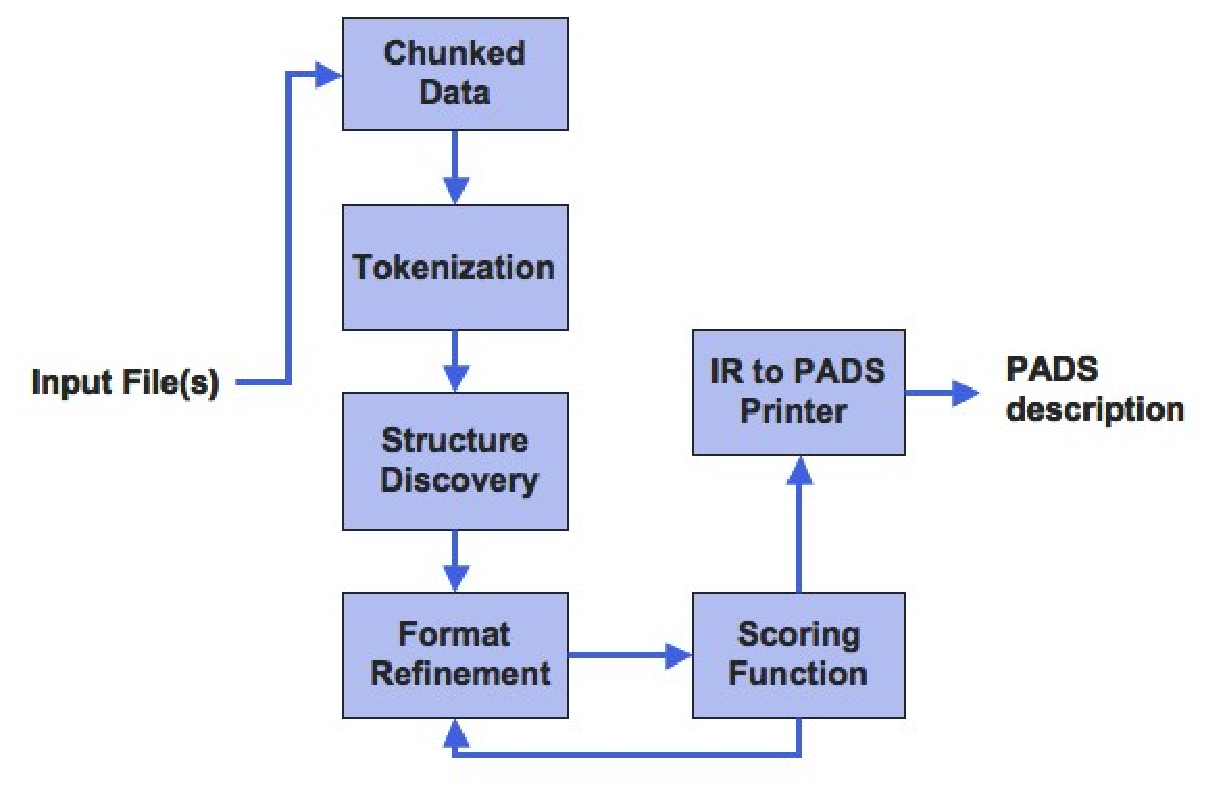
\epsfig{file=archi.eps, width=\columnwidth}
\caption{Architecture of the format inference engine}
\label{fig-archi}
\end{center}
\end{figure}
Figure \ref{fig-archi} gives the big picture of the format inferencing
architecture. The input data, or the ``training set'', 
is first ``chunked'' into records where
each record is often a piece of recurrent data such as a line, 
a paragraph or even a file (if the input consists of multiple files).
Each record is then broken down into a series of tokens where each
token can be a number, a date, a time using a regular expression
based tokenization scheme. In the structure discovery phase,
frequency distribution of each type of tokens is examined, and
a rough structure is discovered in a recursive manner. The idea here 
is similar to \cite{arasu+:sigmod03}. This
rough structure is represented by an intermediate representation or
IR, which has similar expressive power as the \pads{} language. 

The format refinement step refines the IR by applying a number of
rewrite rules sequentially. This is equivalent to a local search
procedure aimming at improving the ``quality'' of the inferred formmat.
The quality is measured by a scoring function which is based on the
information theory. The objective of this function is to
minimize the cost of transmitting the inferred format plus the
training set. The refinement step loops until there is no possible
improvement in the score. Below is an example IR for the web log
data above.

{\small
\begin{verbatim}
Pstruct(Id = BTy_29 6)
        [IP] (Id = BTy_0 6);
        [StringConst] " - - [" (Id = BTy_1 6);
        [Date] (Id = BTy_7 6);
        [StringConst] ":" (Id = BTy_8 6);
        [Time] (Id = BTy_9 6);
        [StringConst] "] "" (Id = BTy_10 6);
        [Enum] {[StringConst] "GET", 
		[StringConst] "POST"} 
        [StringConst] " " (Id = BTy_15 6);
        [Path] (Id = BTy_16 6);
        [StringConst] " HTTP/" (Id = BTy_17 6);
        [Pfloat] (Id = BTy_20 6);
        [StringConst] "" " (Id = BTy_23 6);
        [IntConst] [200] (Id = BTy_26 6);
        [StringConst] " " (Id = BTy_27 6);
        [Pint] (Id = BTy_28 6);
End Pstruct
\end{verbatim}
}

The IR is a tree structure where each if its node is a type.
We include auxilary information such as labels of the nodes
and the number of records covered by a node in the IR to assist
the rewriting. Finally, the refined IR is translated
by a ``pretty printer'' into a PADS program like this which will
then lead to the suite of useful tools:

{\small
\begin{verbatim}
Penum Enum_14 {
        GET14 Pfrom("GET"),
        POST14 Pfrom("POST")
};
Precord Pstruct Struct_29 {
        Pip var_0;
        " - - [";
        Pdate var_7;
        ':';
        Ptime var_9;
        "] \"";
        Enum_14 var_14;
        ' ';
        Ppath var_16;
        " HTTP/";
        Pfloat64 var_20;
        "\" ";
        Puint8 var_26 : var_26 == 200;
        ' ';
        Pint64 var_28;
};
Psource Parray entries_t {
        Struct_29[];
};
\end{verbatim}
}

\bibliography{main}
\bibliographystyle{mlapa}

\end{document} 
